\chapter{Constructive Heuristics}

\section{Greedy}\label{sec:greedy}
Greedy heuristic for TSP start by choosing a random element and add always the closer node, one node at a time, making the local optimal choice. This create good path in the first part of the tour, however the last added edges create different crosses. Therefore this heuristic can be applied in combination with refining heuristics such as: \texttt{local\_branching}, \texttt{hard\_fixing}, \texttt{best\_two\_opt} and other ones that try to improve a tour.\\
The algorithm computational time is $ O(n^2) $ where $ n = |V| $, therefore is pretty fast, however depending on the first selected node, the cost of the tour can differ more than 10 \% one another. The implemented algorithm (from now only \texttt{Greedy} or \texttt{heuristic\_greedy}), at cost of execution time, perform the described greedy using all the nodes as starting node, returning the shortest tour. The time complexity for the implemented algorithm raise to $ O(n^3) $.\\
In fig \ref{fig:a280_10_} an example of tour calculated with the implemented algorithm.

\begin{figure}[h]
	\centering
	\centering
	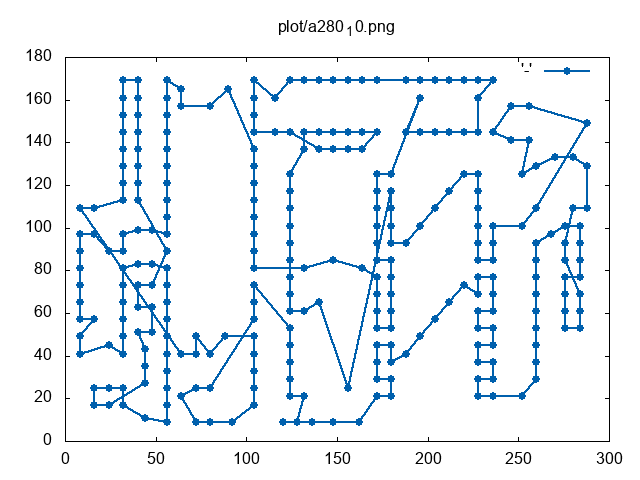
\includegraphics[width=0.7\columnwidth]{../res/a280_10.png}
	\caption{The shortest greedy tours.}
	\label{fig:a280_10_}
\end{figure}



\subsection{Greedy with CGAL Library}
To take a look at the potential of the CGAL library, we decided to implement the greedy algorithm. It follows the same idea as the one previously described (Section \ref{sec:greedy}) but using completely different data structures. Thanks to the potential of the C++ code and therefore the use of objects, the CGAL library offers a very wide range of elements.\\ 
The installation of CGAL within the Windows environment with Visual Studio 2019 is reported in the appendix \ref{sec:cagalOne}.\\
First of all, the objects used for this algorithm are briefly explained:
\begin{enumerate}
\item \texttt{CGAL::Simple\_cartesian <double> K}: The layer of geometry kernels provides basic geometric entities of constant size and primitive operations on them. Each entity is provided as both a stand-alone class, which is parameterized by a kernel class, and as a type in the kernel class. CGAL provides different kernels, they can differ by internal representation of objects (e.g. cartesian versus homogeneous) or provide different functionalities. When creating a new package, the authors have to specify clearly the requirements needed by the kernel used and may specify a targeted kernel in the list of predefined kernels. In this project \texttt{Exact\_predicates\_inexact\_constructions\_kernel} is used. Thus, a \texttt{Simple\_cartesian} object is chosen to represent a model for a kernel using Cartesian coordinates to represent the geometric objects.
\item \texttt{CGAL::Search\_traits\_2 <K> TreeTraits}: The \texttt{Simple\_cartesian} allows to define a dD Spatial Searching which is, in this kind of problems, a 2D space.
\item \texttt{CGAL::Orthogonal\_k\_nemap.com\_search <TreeTraits> Neighbor\_search}: Thanks to the aforementioned objects, with this one a neighborhood search is created, based on the Euclidean distance in a Cartesian plane.
\item \texttt{Neighbor\_search::Tree Tree}: In our implementation was decided to use a Tree representation in which to apply the \texttt{Neighbor\_search}.
\end{enumerate}
Once the model and structure have been defined, the search is simple. Each node is created via the \texttt{Point\_2} object of the kernel defined above. The various points are assigned to the \texttt{Tree}. As a last step just pass: the \texttt{Tree}, the starting node and the number of total nodes to the \texttt{Neighbor\_search} and it return an list of nodes in ascending order of distance from the starting one.\\
By repeating this procedure for each node, a matrix of nodes sorted by distance from the starting point is obtained and with an ad hoc searching function:

\begin{lstlisting}
vector<int>::iterator it = find_if(neigh_sol_idx[succ].begin(), neigh_sol_idx[succ].end(),
					 [&](int neig) {
	return find(var->sol[i].begin(), var->sol[i].end(), neig) == var->sol[i].end();
});
\end{lstlisting}

the resulting matrix will have a number of lines equal to the number of nodes and each of them will be a tour built starting from a node and always choosing the closest from the current node, exactly as \texttt{Greedy}. \\
The algorithm, as shown in fig. \ref{fig:Lconstructives_time} , takes longer to run, as it uses higher level objects and methods than \texttt {Greedy}. In fact, its potential lies in its application in complex problems, in which these data structures offer powerful and effective tools for geometric problems.

\section{Greedy Randomize Adaptive Search Path (GRASP)}\label{sec:grasp}
GRASP heuristic, as the name anticipate, is a Greedy constructive heuristic with some randomization. Indeed, for the TSP problem, instead of bringing the closer isolated node as next, it's chosen a random one between the first $ n $ closest isolated nodes, where $ n = 3 $ in the tested implementation.
The idea is that in TSP it's not always the closer to be the next node on the optimum tour. Moreover, in other metaheuristics that start from a solution and optimize it, a percentage of randomness could appreciated.

\begin{figure}[!h]
	\centering
	\begin{subfigure}{.75\textwidth}
		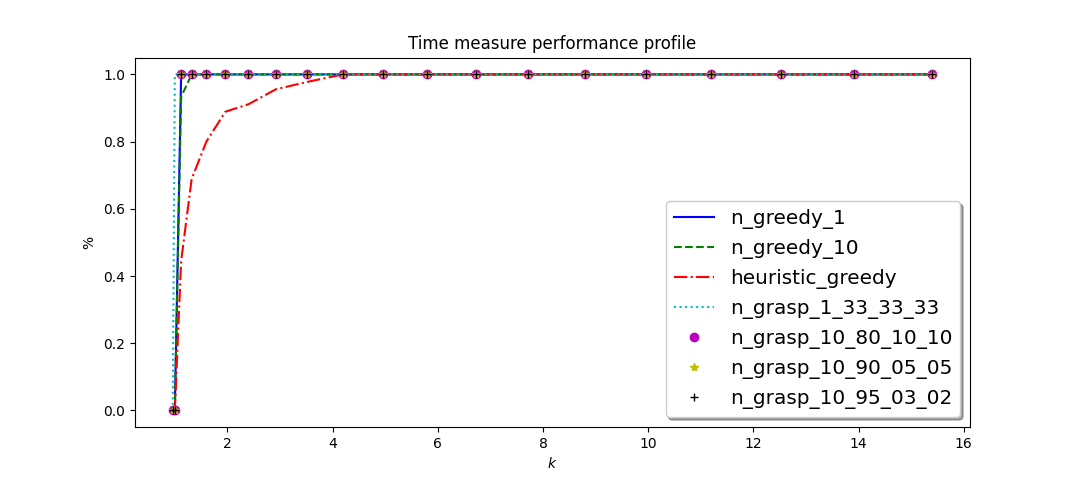
\includegraphics[width=\columnwidth]{../res/Lgrasp_greedy_time.png}
		\caption{}
		\label{fig:Lgrasp_greedy_time}
	\end{subfigure}
	\begin{subfigure}{.75\textwidth}
		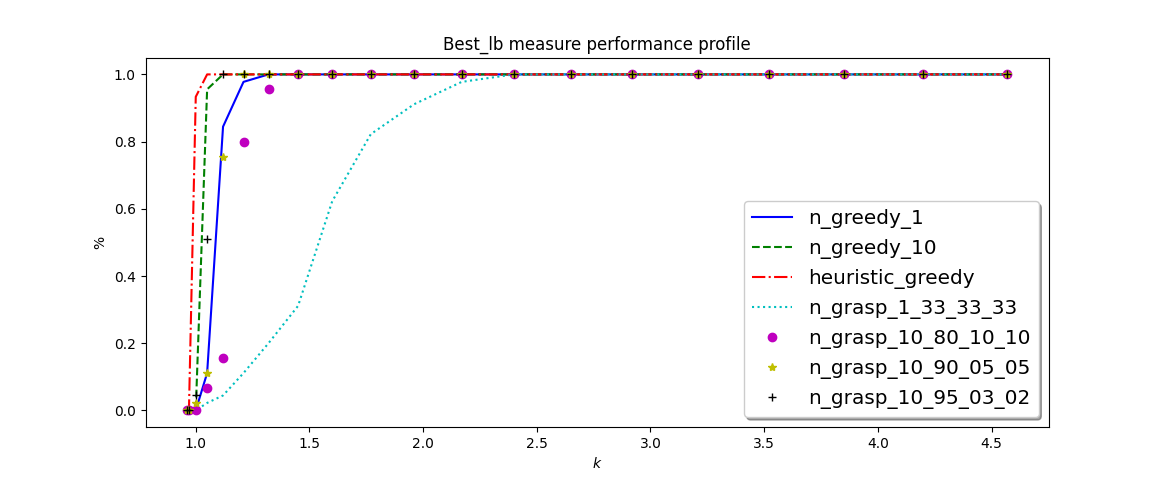
\includegraphics[width=\columnwidth]{../res/Lgrasp_greedy_lb.png}
		\caption{}
		\label{fig:Lgrasp_greedy_lb}
	\end{subfigure}
\caption{The first parameter in the name of \texttt{n\_greedy} and \texttt{n\_grasp} is the number of different tour evaluated. In \texttt{n\_grasp} name the other parameter represent the probability to chose in order the first, the second and the third closer node.  }
\label{fig:Lgrasp_greedy}
\end{figure}
In fig. \ref{fig:Lgrasp_greedy} the result of the test with different $ n $ values for \texttt{n\_greedy} and \texttt{n\_grasp} and for different probability of choice of the next node in \texttt{n\_grasp}. There can be see the differences in execution time of \texttt{heuristic\_greedy} from the other and the gradual decrease of the cost of the \texttt{n\_grasp} by increasing the probability to select the closer node until \texttt{n\_greedy\_10}    

In figure \ref{fig:att48_diff} can be compared of the optimum tour, \texttt{Greedy}, 3 different instances of \texttt{GRASP} (\texttt{n\_grasp\_1 \\ \_33\_33\_33} version) and \texttt{heuristic\_insertion}. It's nice to see that the \texttt{Greedy} (fig \ref{fig:att48_GREEDY}) is pretty close to the optimal solution and also some instance of \texttt{GRASP} like \ref{fig:att48_GRASP2}. \texttt{heuristic\_insertion} in this example has no cross edges and as will be show in fig. \ref{fig:Lgrasp_insertion_refining_LA_lb} the refining phase of this solutions does not improve so much the tour cost.
\begin{figure}[!h]
	\begin{subfigure}{.49\textwidth}
		\centering
		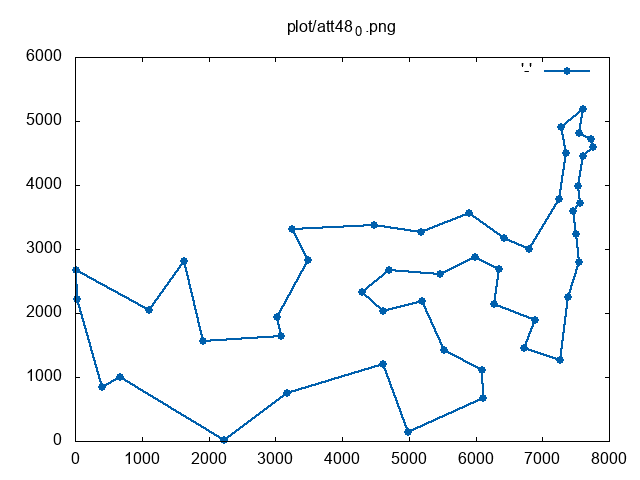
\includegraphics[width=\columnwidth]{../res/att48_0.png}
		\caption{Optimal subtour: cost=10628, time=0.76s}
		\label{fig:att48_best}
	\end{subfigure}
	\begin{subfigure}{.49\textwidth}
		\centering
		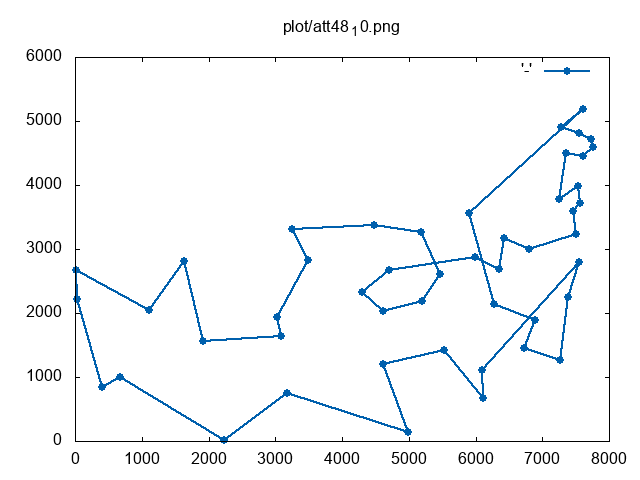
\includegraphics[width=\columnwidth]{../res/att48_10.png}
		\caption{\texttt{Greedy}: cost=12012, time=0.005s}
		\label{fig:att48_GREEDY}
	\end{subfigure}
	\begin{subfigure}{.49\textwidth}
	\centering
	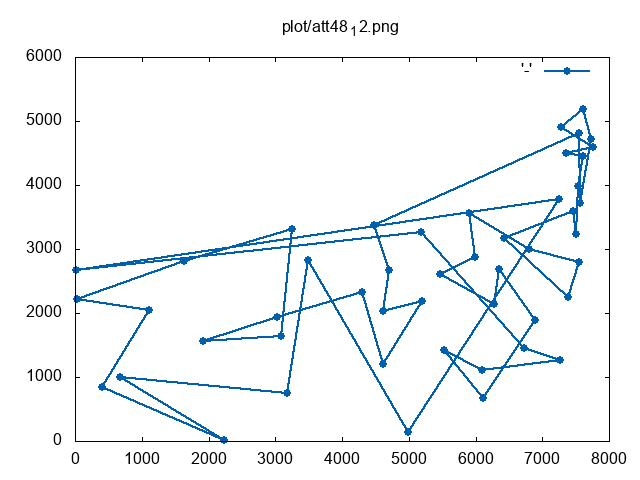
\includegraphics[width=\columnwidth]{../res/att48_12_1.png}
	\caption{\texttt{GRASP}: cost=21824, time=0.001s}
	\label{fig:att48_GRASP1}
	\end{subfigure}
	\begin{subfigure}{.49\textwidth}
	\centering
	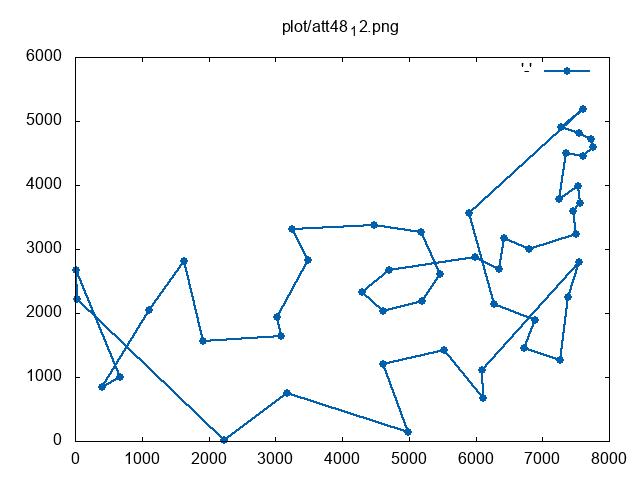
\includegraphics[width=\columnwidth]{../res/att48_12_2.png}
	\caption{\texttt{GRASP}: cost=12576, time=0.001s}
	\label{fig:att48_GRASP2}
	\end{subfigure}
	\begin{subfigure}{.49\textwidth}
	\centering
	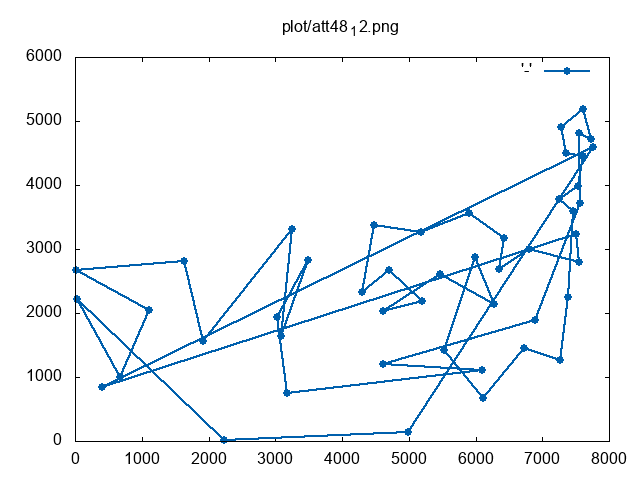
\includegraphics[width=\columnwidth]{../res/att48_12_3.png}
	\caption{\texttt{GRASP}: cost=22179, time=0.001s}
	\label{fig:att48_GRASP3}
	\end{subfigure}
	\begin{subfigure}{.49\textwidth}
	\centering
	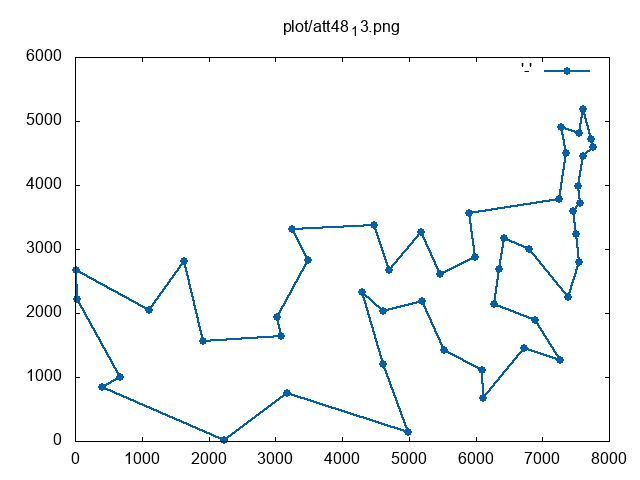
\includegraphics[width=\columnwidth]{../res/att48_13.png}
	\caption{\texttt{heuristic\_insertion}: cost=11197, time=0.0028s}
	\label{fig:att48_insertion}
	\end{subfigure}
	\caption{Differences of \texttt{Greedy} and \texttt{GRASP} tour for \textit{att48.tsp} instace.}
	\label{fig:att48_diff}
\end{figure}


\section{Insertion Heuristic}
The idea of this constructive heuristic is to create an initial simple tour of 3 nodes randomly and insert one node at a time, breaking the edge that minimize the final tour cost.\\
The complexity of the algorithm is $ O(n^2) $.


\textbf{Construction heuristic comparison.} The performance profile in fig \ref{fig:pp_Lconstructives} show the three constructive presented in this chapter. In particular \texttt{heristic\_insertion} is comparable with \texttt{heuristic\_greedy} in execution time, however it usually find shorter tours of all the other constructive.\\
Other consideration about the constructive heuristics in chapter \ref{chapter:refining}.

\begin{figure}[!h]
	\centering
	\begin{subfigure}{.9\textwidth}
		\centering
		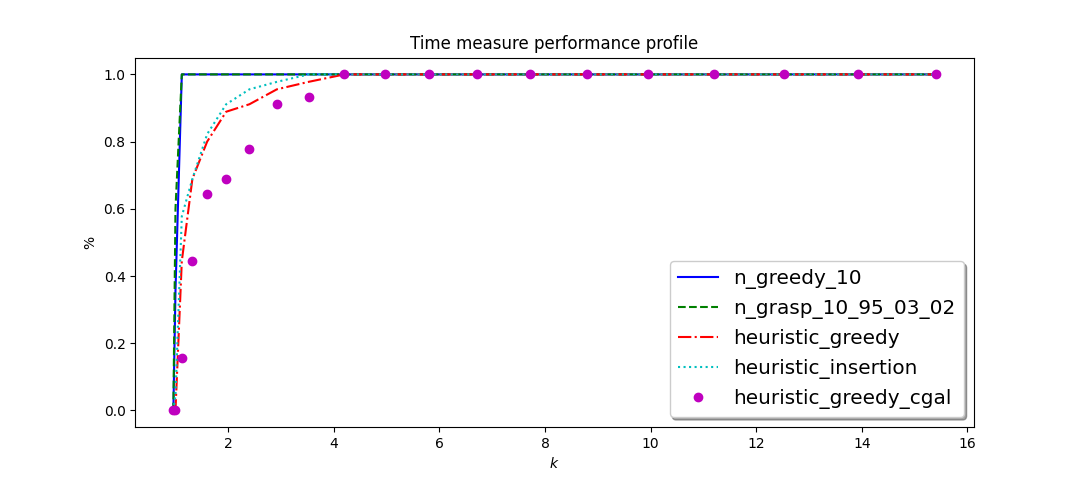
\includegraphics[width=\columnwidth]{../res/Lconstructives_LA_time.png}
		\caption{Solution time domain.}
		\label{fig:Lconstructives_time}
	\end{subfigure}
	\begin{subfigure}{.9\textwidth}
	\centering
	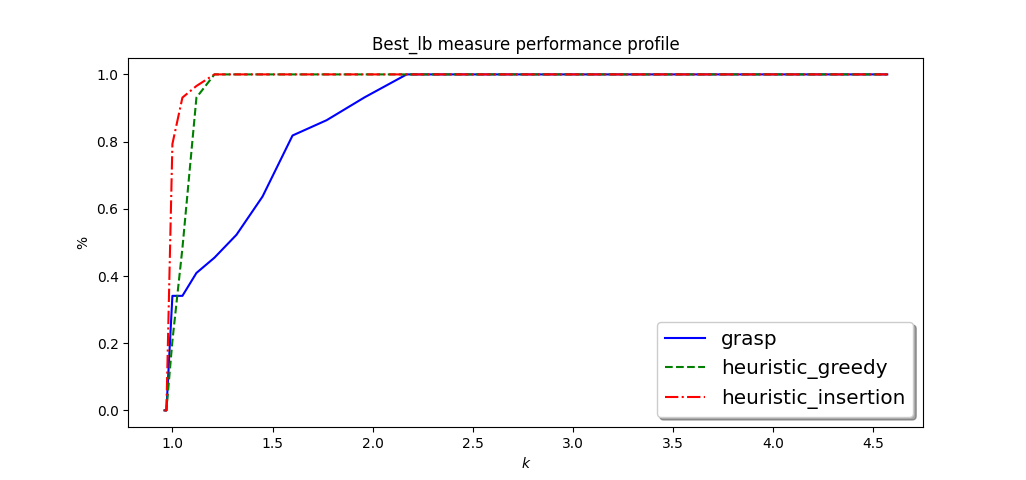
\includegraphics[width=\columnwidth]{../res/Lconstructives_LA_lb.png}
	\caption{Solution cost domain.}
	\label{fig:Lconstructives_lb}
	\end{subfigure}
	\caption{Performance profile of constructive heuristic}
	\label{fig:pp_Lconstructives}
\end{figure}
